\begin{thmBox}{34.1 (Urysohn Metrization Theorem)}[thm:34.1]
    Every regular space \( X \) with a countable basis is metrizable.

    \baseRule

    \begin{proofBox}
        We shall prove that \( X \) is metrizable by imbedding \( X \) in a 
        metrizable space \( Y \); that is, by showing that \( X \) is homeomorphic
        with a subspace of \( Y \).
        There are two version of this proof, and they differ in the choice of the 
        metrizable space \( Y \).
        In the first version, \( Y \) is the space \( \mathbb{R}^{ \omega } \) in the
        product topology, a space that we have previously proved to be metrizable
        (Theorem 20.5). In the second version, the space \( Y \) is also 
        \( \mathbb{R}^{ \omega } \), but this time in the topology given by the
        uniform metric \( \overline{ \rho } \) (see \S 20). In each case, it turns
        out that our construction actually imbeds \( X \) in the subspace 
        \( [ 0, 1 ]^{ \omega } \) of \( \mathbb{R}^{ \omega } \).

        \baseSkip

        We shall focus on the first version of the proof and want to prove the 
        following:
        \begin{center}
            There exists a countable collection of continuous functions
            \( f_{ n }: X \rightarrow [ 0, 1 ] \) having the property that given any
            point \( x_{ 0 } \) of \( X \) and any neighborhood \( U \) of 
            \( x_{ 0 } \), there exists an index \( n \) such that \( f_{ n } \) is 
            positive at \( x_{ 0 } \) and vanishes outside \( U \).
        \end{center}
        Notice that because we are given \( X \) to be regular and second-countable,
        it follows by [\hyperlink{thm:32.1}{Theorem 32.1}] that \( X \) is normal.
        
        \baseSkip

        Let \( \mathcal{B} = \{ B_{ n } \} \) be a countable basis for \( X \).
        For each pair \( n, m \) of indices for which 
        \( \overline{ B }_{ n } \subset B_{ m } \), we can apply the 
        [\hyperlink{thm:33.1}{Urysohn Lemma}] to choose a continuous function
        \( g_{ n, m }: X \rightarrow [ 0, 1 ] \) such that 
        \begin{equation*}
            g_{ n, m } ( \overline{ B }_{ n } ) = \{ 1 \}
            \quad \mathrm{and} \quad 
            g_{ n, m } ( X \setminus B_{ m } )
            =
            \{ 0 \}
        \end{equation*}
        We shall now define \( \mathcal{G} = \{ g_{ n, m } \} \).

        \baseSkip

        We can see that \( \mathcal{G} \) satisfies the property that we're after:
        given any \( x_{ 0 } \) of \( X \) and any neighborhood \( U \) of 
        \( x_{ 0 } \), we see that there exists some basis element \( B_{ m } \)
        such that \( x \in B_{ m } \subset U \).
        Because we know that \( X \) is regular, it follows by 
        [\hyperlink{lem:31.1}{Lemma 31.1}] that there exists some open neighborhood 
        \( V \) of \( x_{ 0 } \) such that \( \overline{ V } \subset B_{ m } \).
        Because \( \mathcal{B} \) is a basis for \( X \), we see that there exists 
        some \( B_{ n } \in \mathcal{B} \) such that \( x \in B_{ n } \subset V \).
        Hence, it follows that \( \overline{ B }_{ n } \subset \overline{ V } \),
        which results in \( \overline{ B }_{ n } \subset B_{ m } \)..
        Then, we see that \( n, m \) is a pair of indices for which the function
        \( g_{ n, m } \) is defined, which we know is positive at \( x_{ 0 } \)
        (in fact, it is \( 1 \)) and vanishes outside \( U \) (as 
        \( X \setminus U \subset X \setminus B_{ m } \), and we know that 
        \( g_{ n, m } ( X \setminus B_{ m } ) = \{ 0 \} \)).
        Furthermore, we can see that \( \mathcal{G} \) is countable since the 
        collection \( \{ g_{ n, m } \} \) is indexed with a subset of
        \( \mathbb{Z}_{ + } \times \mathbb{Z}_{ + } \), which we know is countable.
        Therefore, we see that it can be reindexed with the positive integers,
        giving us the desired collection \( \{ f_{ n } \} \).

        \baseSkip

        By the [\hyperlink{thm:34.2}{Imbedding Theorem}], we see that the function
        \( F: X \rightarrow \mathbb{R}^{ \omega } \) defined by 
        \begin{equation*}
            F ( x ) = ( f_{ n } )_{ n \in \mathbb{Z}_{ + } }
        \end{equation*}
        is an imbedding of \( X \) in \( \mathbb{R}^{ \omega } \).
        Because \( \mathbb{R}^{ \omega } \) is metrizable, hence any of its subsets
        are also metrizable,
        we see that \( X \) must be metrizable as well -- in fact, because we see that
        since each \( f_{ n } \) maps \( X \) into \( [ 0, 1 ] \) for all 
        \( n \in \mathbb{Z}_{ + } \), we have that \( F \) imbeds \( X \) in 
        \( [ 0, 1 ]^{ \omega } \).
    \end{proofBox}
\end{thmBox}

\begin{thmBox}{34.2 (Imbedding Theorem)}[thm:34.2]
    Let \( X \) be a space in which one-point sets are closed (i.e., \( X \) is closed).
    Suppose that \( \{ f_{ i } \}_{ i \in I } \) is an indexed family of continuous 
    functions \( f_{ i }: X \rightarrow \mathbb{R} \) satisfying the requirement that 
    for each point \( x_{ 0 } \) of \( X \) and each neighborhood \( U \) of 
    \( x_{ 0 } \), there is an index \( i \) such that \( f_{ i } \) is positive at
    \( x_{ 0 } \) and vanishes outside \( U \).
    Then the function \( F: X \rightarrow \mathbb{R}^{ I } \) defined by 
    \begin{equation*}
        F ( x )
        =
        ( f_{ i } ( x ) )_{ i \in I }
    \end{equation*}
    is an imbedding of \( X \) in \( \mathbb{R}^{ I } \). 
    If \( f_{ i } \) maps \( X \) into \( [ 0, 1 ] \) for each \( i \), then \( F \)
    imbeds \( X \) in \( [ 0, 1 ]^{ I } \).

    \baseRule

    \begin{proofBox}
        Our goal is to show that \( F \) is an imbedding.
        Recall that an imbedding is an injection that is homeomorphic to its image.

        \baseSkip

        To show that \( F \) is continuous, we first see that each of its components
        \( f_{ i } \) are given to be continuous.
        Because \( \mathbb{R}^{ I } \) has the product topology, it follows by 
        [\hyperlink{thm:18.4}{Theorem 18.4}] that \( F \) is continuous.

        \baseSkip

        To show that \( F \) is injective, let us suppose that \( x \neq y \).
        Since we have that \( X \) is \( T_{ 1 } \), we have that both \( \{ x \} \)
        is closed, which makes \( X \setminus \{ x \} \) an open neighborhood of
        \( y \) in \( X \).
        It follows by the requirements of our functions \( f_{ i } \) that there exists 
        some index \( i \) such that 
        \( f_{ i } ( x ) = 0 \) and \( f_{ i } ( y ) > 0 \); therefore, we get have
        \( F ( x ) \neq F ( y ) \).

        \baseSkip

        We now just need to show that \( F \) is a homeomorphism of \( X \) onto
        its image, which is the subspace \( Z = F ( X ) \) of \( \mathbb{R}^{ I } \).
        It is clear to see that \( F \) is a continuous bijection of \( X \) with 
        \( Z \); thus, all that is left to show is that for each open set \( U \) in
        \( X \), the set \( F ( U ) \) is open in \( Z \).
        Let \( z_{ 0 } \) be a point of \( F ( U ) \). 
        We want to find an open set \( W \) of \( Z \) such that 
        \begin{equation*}
            z_{ 0 } \in W \subset F ( U )
        \end{equation*}
        Because we know that \( F \) is a bijection (namely, surjection), we see that 
        there exists some \( x_{ 0 } \in U \) such that \( F ( x_{ 0 } ) = z_{ 0 } \).
        By the requirements of our functions \( f_{ i } \), we see that there exists
        some index \( N \) for which \( f_{ N } ( x_{ 0 } > 0 ) \) and 
        \( f_{ N } ( X \setminus U ) = \{ 0 \} \).
        Take the open ray \( ( 0, + \infty ) \) in \( \mathbb{R} \), and let \( V \)
        be the open set 
        \begin{equation*}
            V
            =
            \mathrm{proj}_{ N }^{ -1 } ( ( 0, + \infty ) )
        \end{equation*}
        of \( \mathbb{R}^{ I } \).
        Let \( W = V \cap Z \); we can see that \( W \) is open in \( Z \) by 
        definition of the subspace topology.

        \begin{figure}[H]
            \centering
            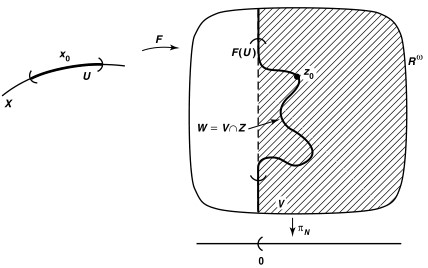
\includegraphics[ width = 0.6\linewidth ]{figures/Section 34/thm34-2jpg.jpg}
            \caption{A visual on \( W \)}
            \label{fig:34-1}
        \end{figure}

        We claim that \( z_{ 0 } \in W \subset F ( U ) \).
        To start, we are given that \( z_{ 0 } \in F ( U ) \subset Z \).
        Notice that 
        \begin{equation*}
            \mathrm{proj}_{ N } ( z_{ 0 } )
            =
            \mathrm{proj}_{ N } ( F ( x_{ 0 } ) ) = f_{ N } ( x_{ 0 } ) > 0
        \end{equation*}
        which tells us that \( z_{ 0 } \in V \); thus, we see that 
        \( z \in ( V \cap Z ) = W \).
        
        \baseSkip
    
        We now want to show that \( W \subset F ( U ) \).
        Let \( z \in W \) be given.
        Since \( F \) is a bijection (namely, a surjection), we see that there exists 
        some \( x \in X \) such that \( z = F ( x ) \).
        Furthermore, we have that \( z \in V \) (by definition of \( W \)), which tells 
        us that \( \mathrm{proj}_{ N } ( z ) \in ( 0, + \infty ) \).
        Since 
        \( 
            \mathrm{proj}_{ N } ( z ) = \mathrm{proj}_{ N } ( F ( x ) ) = f_{ N } ( x ) 
        \),
        it must be that case that \( f_{ N } ( x ) > 0 \).
        Because \( f_{ N } \) vanishes outside \( U \), the point \( x \) must be in 
        \( U \).
        Thus, we see that \( z = F ( x ) \) is in \( F ( U ) \), as desired.
    
        \baseSkip

        Putting everything together tells us that \( F \) is an imbedding of \( X \) in
        \( \mathbb{R}^{ I } \).
    \end{proofBox}
\end{thmBox}

\begin{thmBox}{34.3}[thm:34.3]
    A space \( X \) is completely regular if and only if it is homeomorphic to a 
    subspace of \( [ 0, 1 ]^{ I } \) for some \( I \).

    \baseRule

    \begin{proofBox}

    \end{proofBox}
\end{thmBox}

